\documentclass{article}
\usepackage[utf8]{inputenc}
\usepackage{graphicx}
\usepackage{geometry}
\usepackage{amsmath}
\usepackage{amsfonts}
\usepackage{float}
\usepackage{caption}
\usepackage{subcaption}
\usepackage{enumitem}

\geometry{left=25mm, top=25mm, right=25mm, bottom=25mm}

\title{PHY407 Lab 5}
\author{Pierino Zindel (1002429703) and Hayden Johnson (1002103537)}
\date{October 12, 2018}

\begin{document}

\maketitle

\noindent \textbf{Distribution of work:}

\section{Modeling space garbage (Newman 8.8)}

For this question we desire to model the trajectory of a ball bearing moving around a rod in space. We assume a negligible cross section of the rod and enough mass to avoid movement. Additionally, the trajectory of the ball bearing is taken to be in a plane perpendicular to the rod with $z=0$.

From part a) of exercise 8.8, the two second order odes that describe the orbit of the ball bearing are given as 

\begin{equation}
	\frac{d^2x}{dt^2} = f_x = -GM\frac{x}{r^2\sqrt{r^2 + L^2/4}}
	\label{eq:1}
\end{equation}
and 
\begin{equation}
	\frac{d^2y}{dt^2} = f_y = -GM\frac{y}{r^2\sqrt{r^2 + L^2/4}}
	\label{eq:2}
\end{equation}

where $r=\sqrt{x^2+y^2}$.

The two second-order odes were then converted to four first-order odes with 
\begin{equation}
	\frac{dv_x}{dt} = f_x 
\end{equation}
\begin{equation}
	\frac{dx}{dt} = v_x
\end{equation}
\begin{equation}
	\frac{dv_y}{dt} = f_y 
\end{equation}
\begin{equation}
	\frac{dy}{dt} = v_y 
\end{equation}

The system of equations was then solved using the 4th-order Runge-Kutta method with the initial conditions $x=1$, $y=0$, $v_x=0$, $v_y=1$; constant values $G=1$, $M=10$, $L=2$, and integrated over the interval $0<t<10$ with $1000$ steps. The resulting orbit trajectory of the ball bearing was then plotted and is shown in figure \ref{fig:q1_orbit}. We see that the resulting orbit is not a simple circular orbit but rather a precessing orbit as suggested in the textbook due to the rod having a non-spherical shape.


\begin{figure}[H]
	\centering
	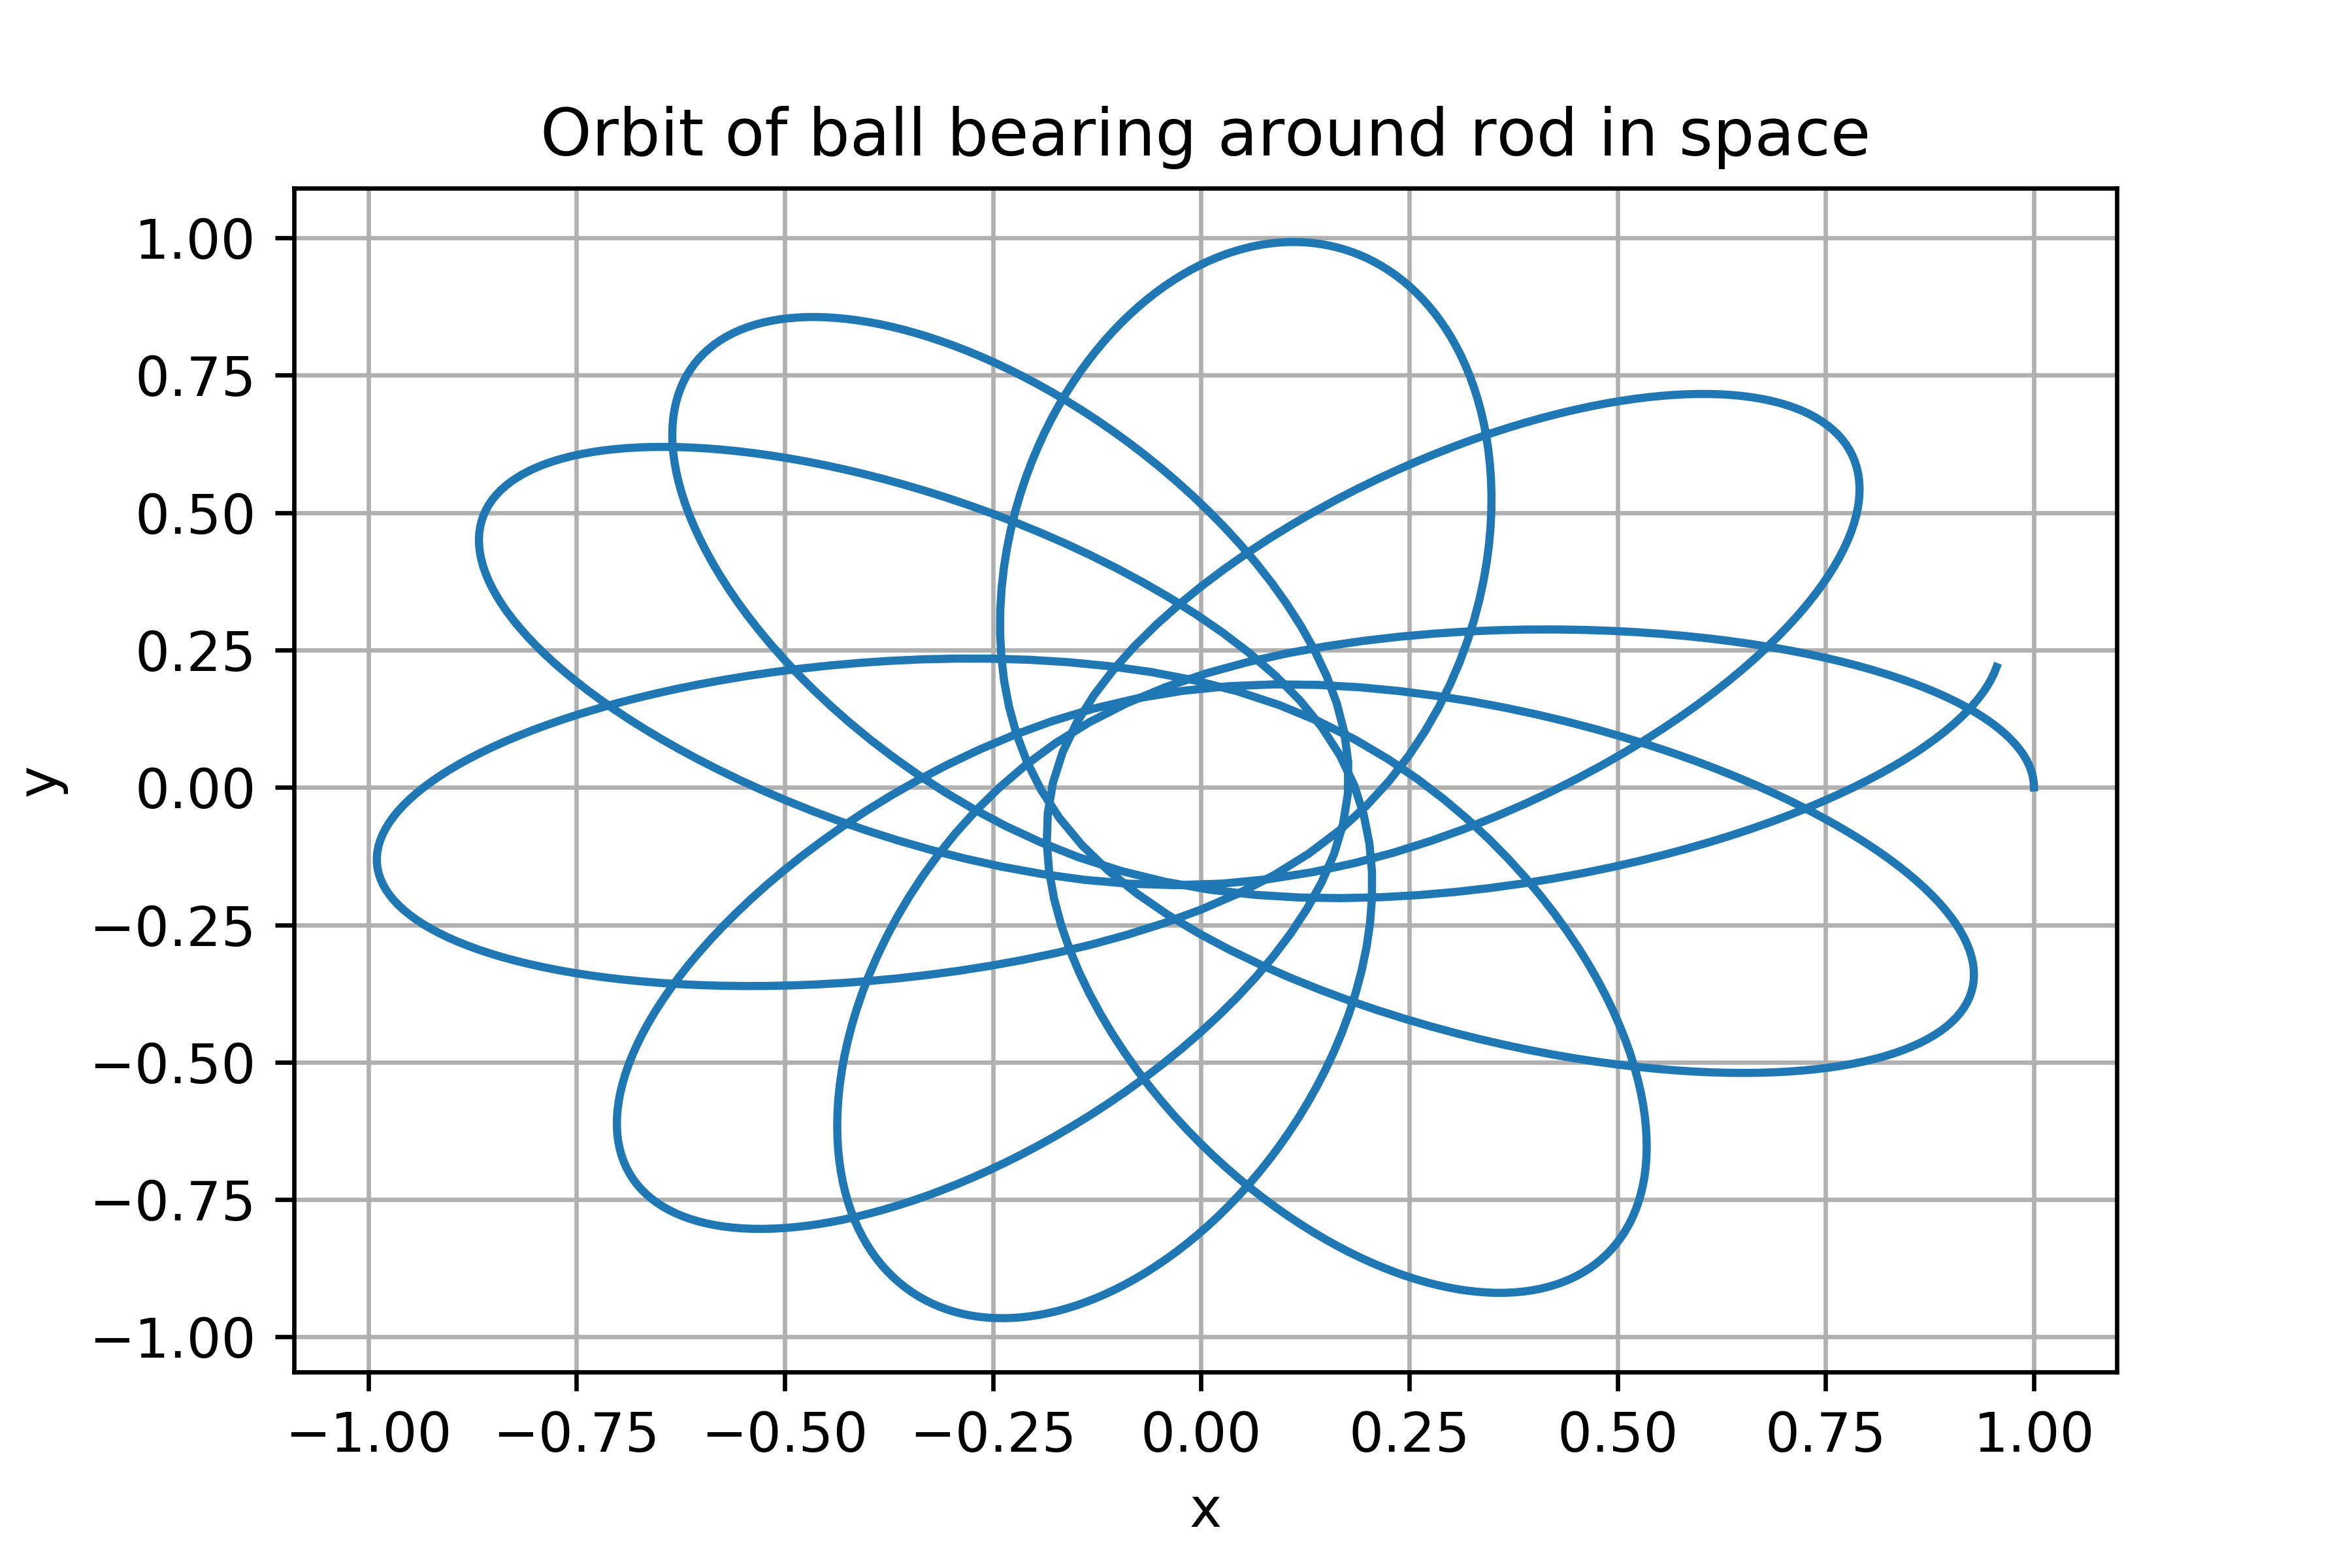
\includegraphics[width=0.8\textwidth]{../images/q1_orbit.png}
	\caption{Precessing orbit of a ball bearing around a rod, in a plane perpendicular to the rod. Equations of motion of the ball given by equations \ref{eq:1} and \ref{eq:2} with initial conditions of $(x,y,v_x,v_y)=(1,0,0,1)$.}
	\label{fig:q1_orbit}
\end{figure}

\section{Molecular Dynamics Simulation Part 1}

\subsection{Part b)}

We seek to write psuedocode, and then an actual program, to compute the trajectories of two particles interacting via the Lennard-Jones potential, and produce plots of the trajectories, for several different sets of initial conditions.

\subsubsection{Pseudocode}

\begin{enumerate}
	\item Define a function to compute the acceleration of each particle as a function of their positions
	\begin{enumerate}[label*=\arabic*]
		\item Compute the x and y distance between the particles
		\item Compute the square of the distance between the two particles
		\item Compute the scalar value of the force acting between the two particles (found by differentiating eq. 12 from the handout with respect to $r$)
		\item Compute the value of the x and y accelerations on each particle
	\end{enumerate}
	\item Input initial positions and velocities of particles
	\item Define timestep and number of steps
	\item Create empty arrays to store position and velocity values at each step; note that the velocity array must be twice as long as the position array, and the data at index $i$ in the position array will correspond to data at index $2i$ in the velocity array
	\item Input initial position and velocity values into first element (along the time axis) of the arrays storing position and velocity
	\item Initialize the velocity values at $t=0.5*h$
	\item Iterate over the length of the position array (index $i$)
	\begin{enumerate}[label*=\arabic*]
		\item Calculate position $i+1$ using eq. 8 from handout
		\item Calculate $\vec{k}$ using eq. 9 from handout and the acceleration function defined earlier
		\item Calculate velocity $2(i+1)$ using eq. 10 from handout
		\item Calculate valocity $2(i+1)+1$ using eq. 11 from handout
	\end{enumerate}
	\item Plot trajectories of the particles
\end{enumerate}

\subsubsection{Plots}

The plots produced for the trajectories of both particles in the case of all three different sets of initial conditions are displayed in figures \ref{fig:q2_i_traj}, \ref{fig:q2_ii_traj} and \ref{fig:q2_iii_traj}. Because it is difficult to tell the direction of motion simply from the trajectory plots, we have also plotted the x position of the particles as a function of time, in figures \ref{fig:q2_i_xpos}, \ref{fig:q2_ii_xpos} and \ref{fig:q2_iii_xpos}. From figure \ref{fig:q2_i_xpos} it is clear that the first initial condition results in the particles oscillating back and forth towards and away from each other, moving gently back and forth between the regimes of attraction at farther distances and repulsion at short distances. Figure \ref{fig:q2_ii_xpos} makes it clear that for the second set of initial conditions, the particles start close enough together to repel each other quite strongly and then simply fly away from each other, evidently overcoming the attractive force felt at farther distances. In the third set of initial conditions, we see from figure \ref{fig:q2_iii_xpos} that the particles slowly start to move towards each other, as a result of the attractive force at large distances.

\begin{figure}[H]
	\centering
	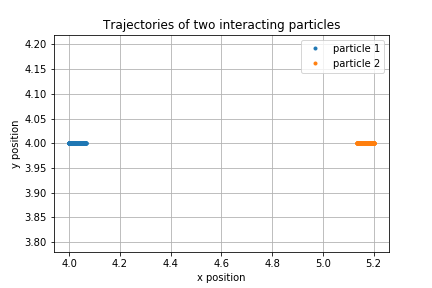
\includegraphics[width=0.8\textwidth]{../images/q2_i_traj.png}
	\caption{Plot of trajectories with initial conditions $\vec{r_1}=(4,4)$, $\vec{r_2}=(5.4,4)$}
	\label{fig:q2_i_traj}
\end{figure}

\begin{figure}[H]
	\centering
	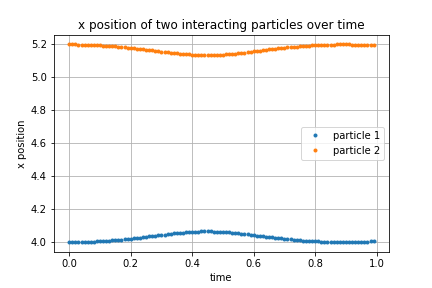
\includegraphics[width=0.8\textwidth]{../images/q2_i_xpos.png}
	\caption{Plot of x positions over time with initial conditions $\vec{r_1}=(4,4)$, $\vec{r_2}=(5.4,4)$}
	\label{fig:q2_i_xpos}
\end{figure}

\begin{figure}[H]
	\centering
	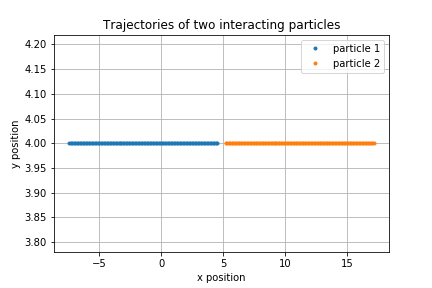
\includegraphics[width=0.8\textwidth]{../images/q2_ii_traj.png}
	\caption{Plot of trajectories with initial conditions $\vec{r_1}=(4.5,4)$, $\vec{r_2}=(5.4,4)$}
	\label{fig:q2_ii_traj}
\end{figure}

\begin{figure}[H]
	\centering
	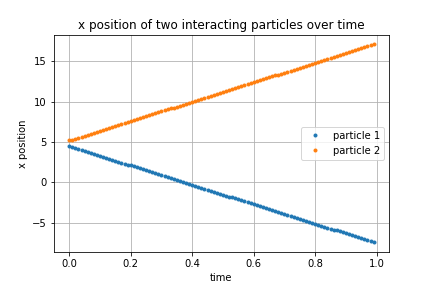
\includegraphics[width=0.8\textwidth]{../images/q2_ii_xpos.png}
	\caption{Plot of x positions over time with initial conditions $\vec{r_1}=(4.5,4)$, $\vec{r_2}=(5.4,4)$}
	\label{fig:q2_ii_xpos}
\end{figure}

\begin{figure}[H]
	\centering
	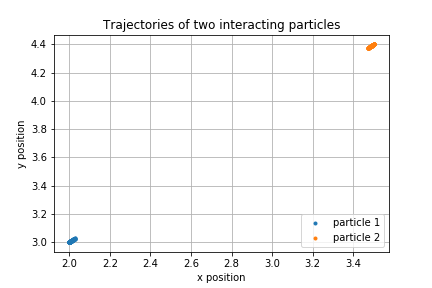
\includegraphics[width=0.8\textwidth]{../images/q2_iii_traj.png}
	\caption{Plot of trajectories with initial conditions $\vec{r_1}=(2,3)$, $\vec{r_2}=(3.5,4.4)$}
	\label{fig:q2_iii_traj}
\end{figure}

\begin{figure}[H]
	\centering
	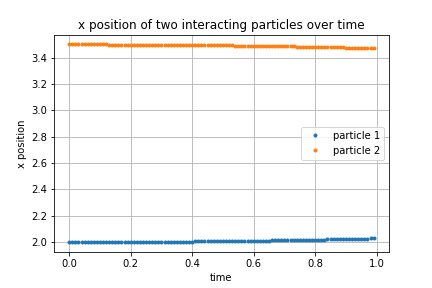
\includegraphics[width=0.8\textwidth]{../images/q2_iii_xpos.png}
	\caption{Plot of x positions over time with initial conditions $\vec{r_1}=(2,3)$, $\vec{r_2}=(3.5,4.4)$}
	\label{fig:q2_iii_xpos}
\end{figure}

\subsection{Part c)}

\section{Molecular Dynamics Simulation Part 2}

\subsection{Part c)}
For this section we desire to modify the results of part b by implementing boundary conditions as defined in the lab manual. To start we added the boundary of $0<x<4$ and $0<y<4$ in such a manner that whenever a particle's component fell outside of these limits the particle would be modulated such that it would reenter the frame from the opposite side. The resulting trajectories are plotted in figure \ref{fig:q3_bdry}. We then attempted to implement the second condition that imposed outside forces on our frame. This condition required us to emulate the particles 8 times in the tiles surrounding our frame and then compute and add the forces of the particles of surrounding tiles to the particles in our center frame. Unfortunately the we were not able to properly implement the second condition fully and got several errors when attempting to do so. We managed to plot the trajectories for the first couple of steps with outside forces, shown in figure \ref{fig:q3_bdry_2}. From this subset we cannot fully describe the paths of the particles but we can infer that now all the particles are effected in such a way that the trajectories behave in a noise manner opposed to figure \ref{fig:q3_bdry} where the corner particles have straight trajectories. In comparison to part b we see that since the particles are confine their paths are more noisey.

\begin{figure}[H]
	\centering
	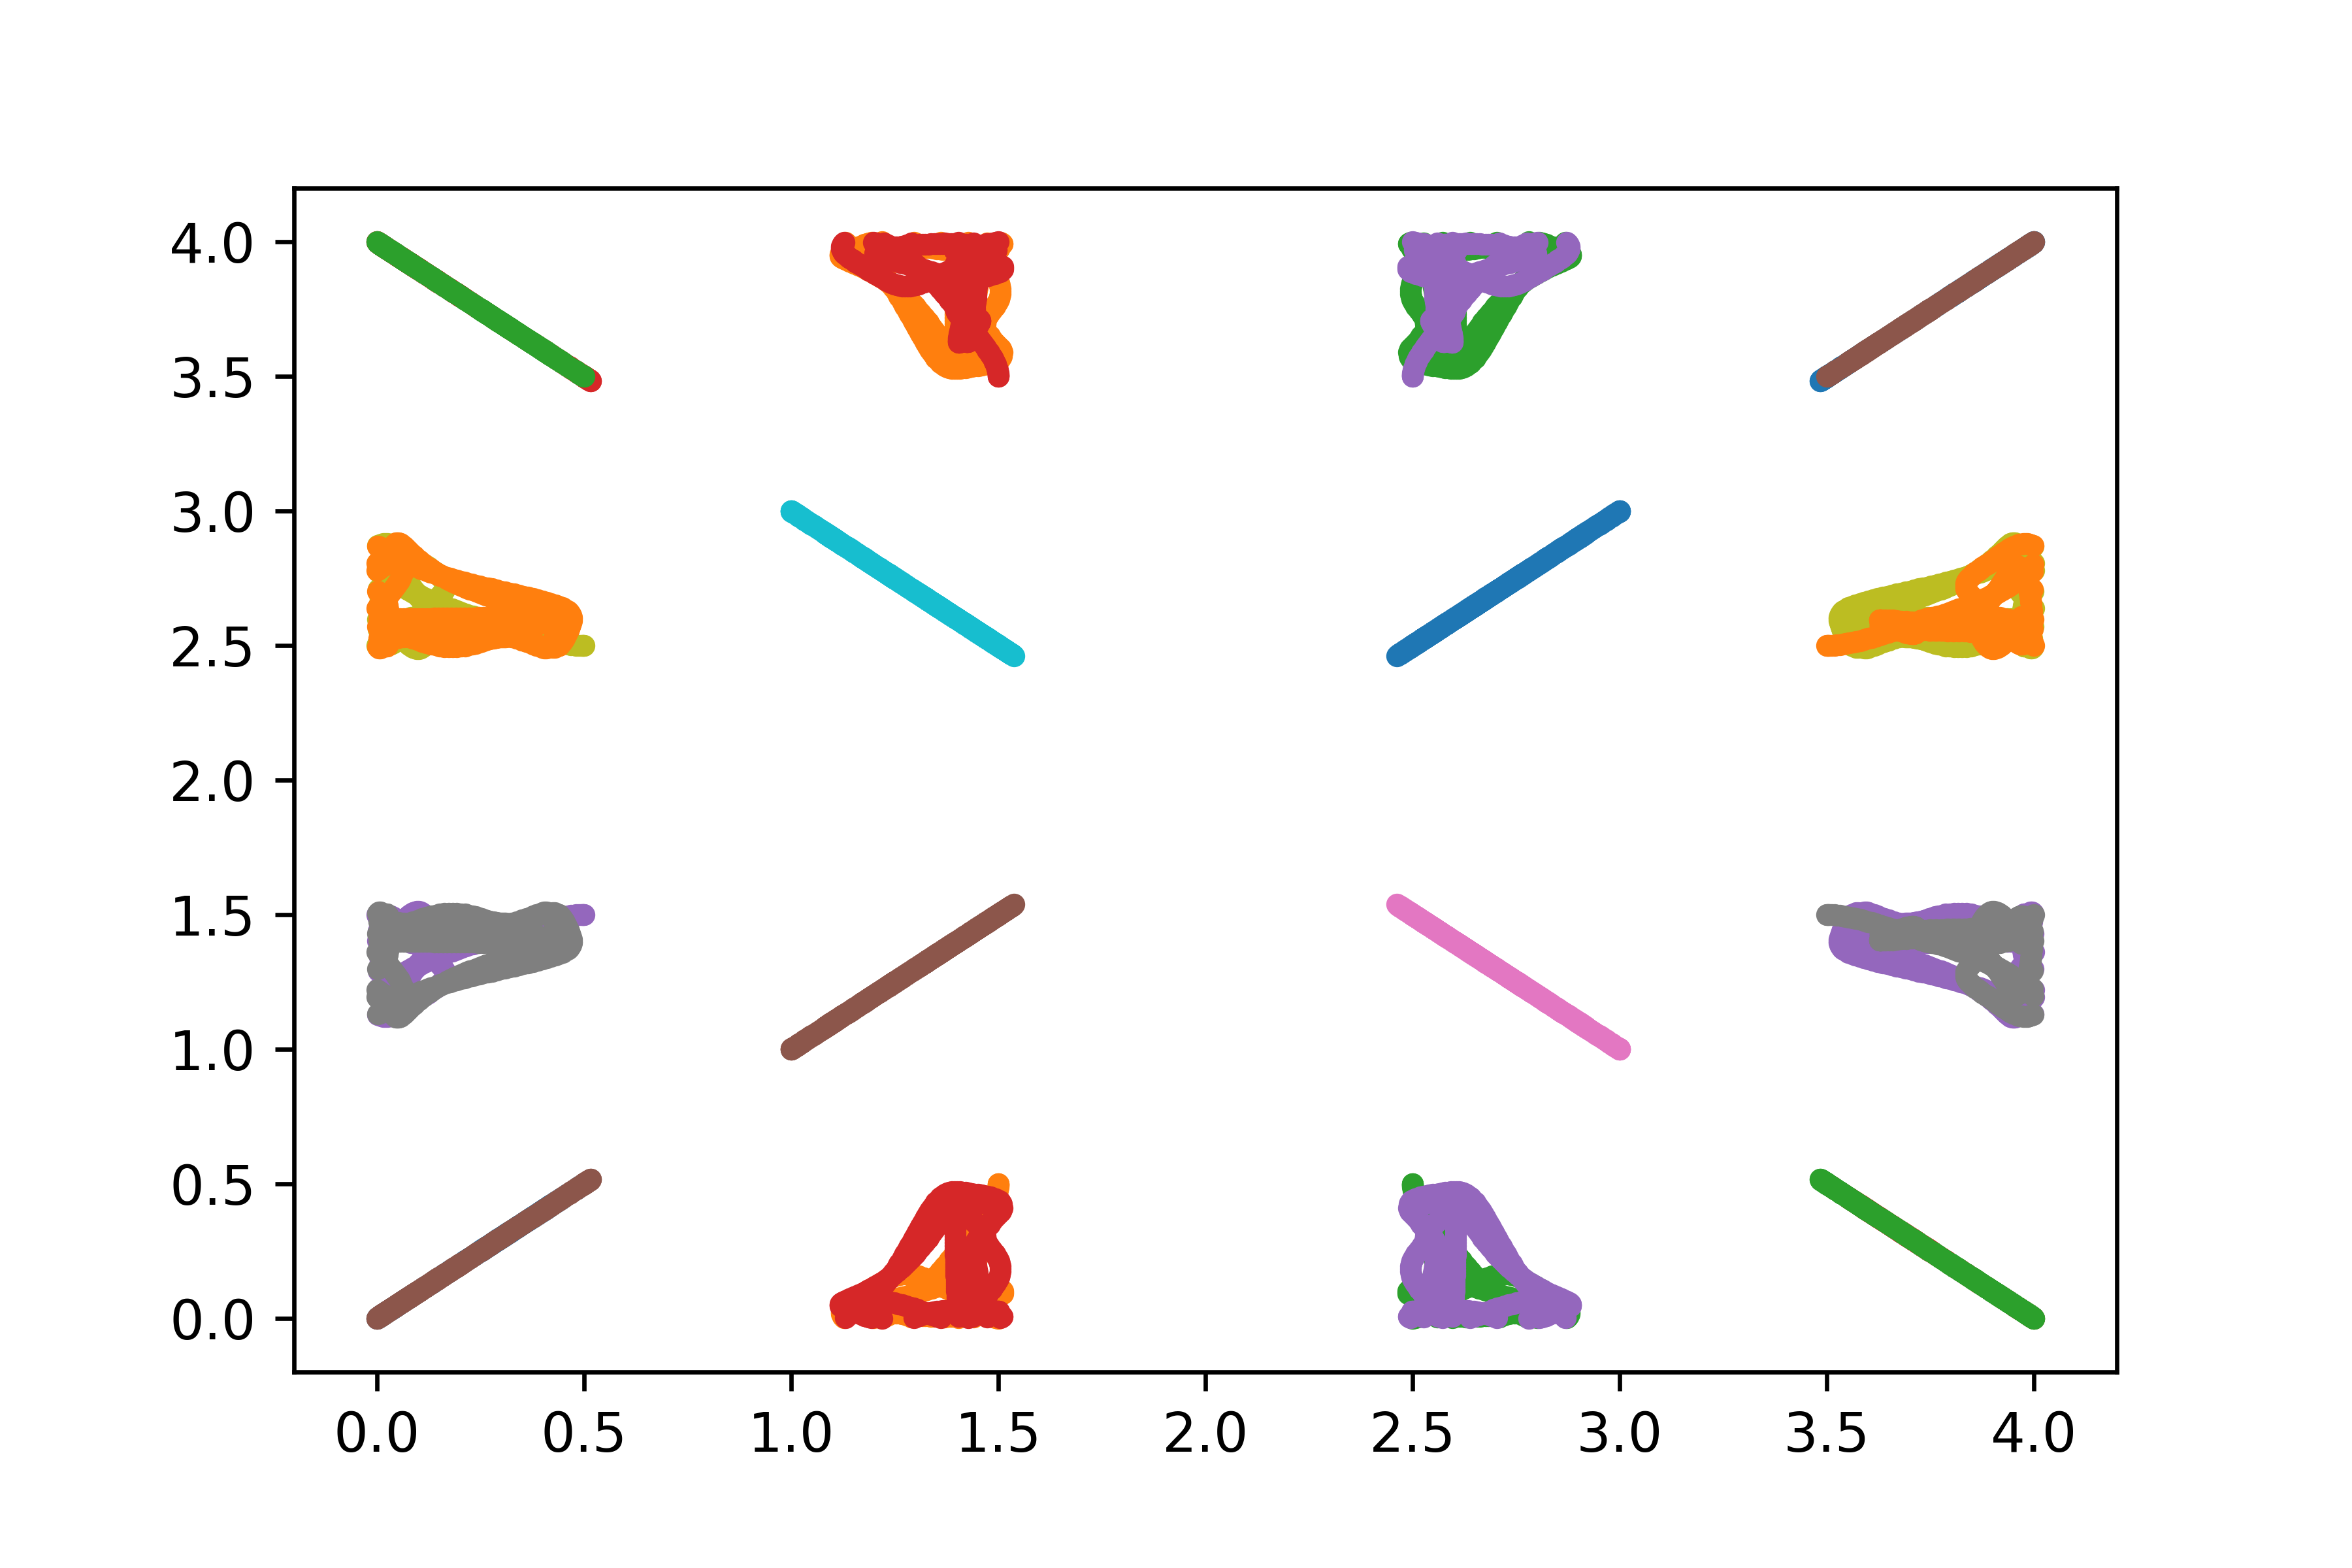
\includegraphics[width=0.8\textwidth]{../images/bdry.png}
	\caption{Plot of trajectories for sixteen particles initially spaced out equally, for 1000 steps with a time step of 0.01 after applying wrap-around boundary conditions.}
	\label{fig:q3_bdry}
\end{figure}

\begin{figure}[H]
	\centering
	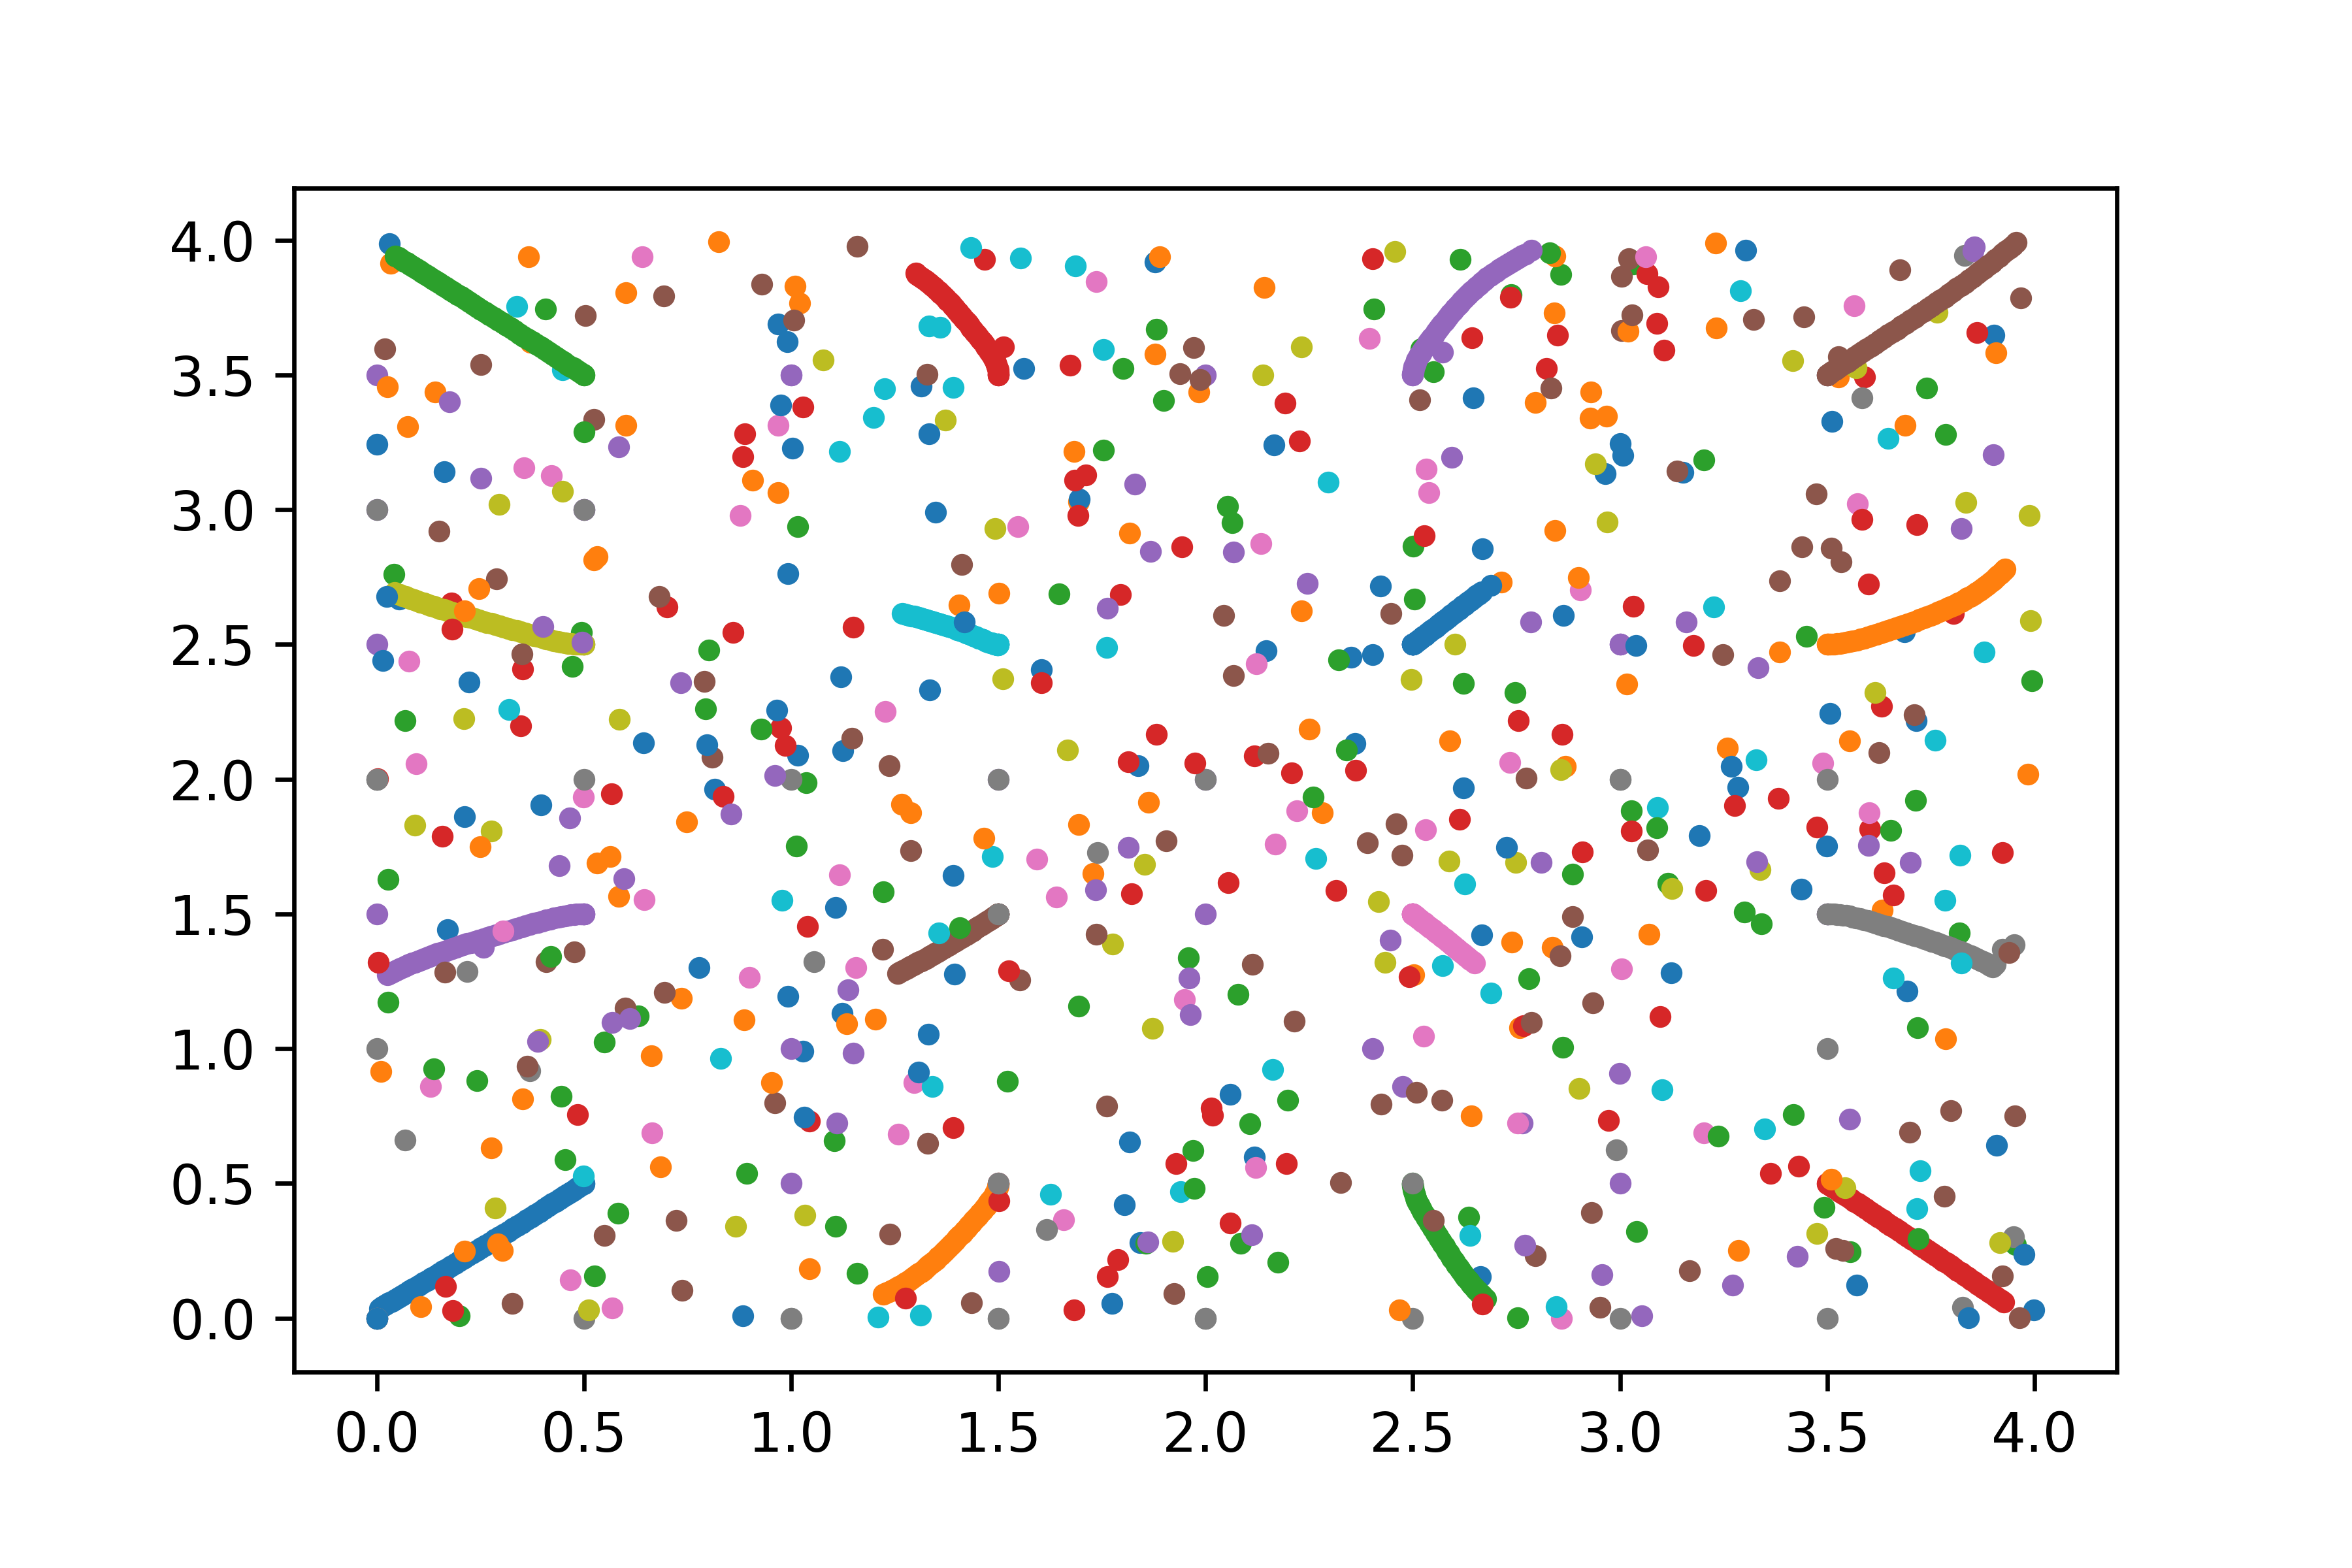
\includegraphics[width=0.8\textwidth]{../images/bdry_2.png}
	\caption{Plot of trajectories for sixteen particles initially spaced out equally, for 1000 steps with a time step of 0.01 after attempting to apply forces from surrounding particles.}
	\label{fig:q3_bdry_2}
\end{figure}


\end{document}
